\documentclass{beamer}
\usepackage[utf8]{inputenc}

\usetheme{Madrid}
\usecolortheme{default}
\usepackage{extarrows}
\usepackage{amsmath}
\usepackage{extarrows}
\usepackage{amssymb,amsfonts,amsthm}
\usepackage{txfonts}
\usepackage{tkz-euclide}
\usepackage{listings}
\usepackage{adjustbox}
\usepackage{array}
\usepackage{tabularx}
\usepackage{gvv}
\usepackage{lmodern}
\usepackage{circuitikz}
\usepackage{tikz}
\usepackage{graphicx}
\usepackage{amsmath} 

\setbeamertemplate{page number in head/foot}[totalframenumber]

\usepackage{tcolorbox}
\tcbuselibrary{minted,breakable,xparse,skins}

\definecolor{bg}{gray}{0.95}
\DeclareTCBListing{mintedbox}{O{}m!O{}}{%
  breakable=true,
  listing engine=minted,
  listing only,
  minted language=#2,
  minted style=default,
  minted options={%
    linenos,
    gobble=0,
    breaklines=true,
    breakafter=,,
    fontsize=\small,
    numbersep=8pt,
    #1},
  boxsep=0pt,
  left skip=0pt,
  right skip=0pt,
  left=25pt,
  right=0pt,
  top=3pt,
  bottom=3pt,
  arc=5pt,
  leftrule=0pt,
  rightrule=0pt,
  bottomrule=2pt,
  toprule=2pt,
  colback=bg,
  colframe=orange!70,
  enhanced,
  overlay={%
    \begin{tcbclipinterior}
    \fill[orange!20!white] (frame.south west) rectangle ([xshift=20pt]frame.north west);
    \end{tcbclipinterior}},
  #3,
}
\lstset{
    language=C,
    basicstyle=\ttfamily\small,
    keywordstyle=\color{blue},
    stringstyle=\color{orange},
    commentstyle=\color{green!60!black},
    numbers=left,
    numberstyle=\tiny\color{gray},
    breaklines=true,
    showstringspaces=false,
}
\title %optional
{5.2.51}

\author 
{EE25BTECH11049-Sai Krishna Bakki}

\begin{document}

\frame{\titlepage}
\begin{frame}{Question}
    Solve the following system of linear equations.
    \begin{align*}
        5x+2y &= 4
    \end{align*}
    \begin{align*}
        7x + 3y &= 5
    \end{align*}
\end{frame}

\begin{frame}{Theoretical Solution}

The equation of line $L_1$ is,
\begin{align}
    \myvec{5 & 2}\vec{x} = 4
\end{align}
The equation of line $L_2$ is,
\begin{align}
    \myvec{7 & 3}\vec{x} = 5
\end{align}

\end{frame}
\begin{frame}{Theoretical Solution}

On putting the equations in a matrix, we will get
\begin{align}
    \implies \myvec{5 & 2\\7 & 3}\vec{x} = \myvec{4\\5}
\end{align}
So the augmented matrix is,
\begin{align}
    \augvec{2}{1}{5 & 2 & 4\\7 & 3 & 5}
\end{align}
\end{frame}

\begin{frame}{Theoretical Solution}
\begin{align}
    \augvec{2}{1}{5 & 2 & 4\\7 & 3 & 5}s\xleftrightarrow[]{R_2\rightarrow R_2-\frac{7}{5}R_1}\augvec{2}{1}{5 & 2 & 4\\0 & \frac{1}{5} & \frac{-3}{5}}
\end{align}
\begin{align}
    \augvec{2}{1}{5 & 2 & 4\\0 & \frac{1}{5} & \frac{-3}{5}}\xleftrightarrow[]{R_2\rightarrow 5R_2}\augvec{2}{1}{5 & 2 & 4\\0 & 1 &-3}
\end{align}
\begin{align}
   \augvec{2}{1}{5 & 2 & 4\\0 & 1 & -3}\xleftrightarrow[]{R_1\rightarrow R_1-2R_2}\augvec{2}{1}{5 & 0 &10 \\0 & 1 & -3}
\end{align}
\end{frame}

\begin{frame}{Theoretical Solution}

\begin{align}
   \augvec{2}{1}{5 & 0 & 10\\0 & 1 & -3}\xleftrightarrow[]{R_1\rightarrow \frac{1}{5}R_1}\augvec{2}{1}{1 & 0 & 2\\0 & 1 & -3}
\end{align}
\begin{align}
    \implies\vec{x} = \myvec{2\\-3}
\end{align}
Therefore the two lines will intersect at \myvec{2\\-3}.
\end{frame}
\begin{frame}[fragile]
\frametitle{C Code}
\begin{lstlisting}
#include <stdio.h>
#include <math.h> // Required for fabs()

// This function solves a system of two linear equations using an augmented matrix
// and Gaussian elimination.
// a*x + b*y = e
// c*x + d*y = f
void solve_system(double a, double b, double c, double d, double e, double f, double* x, double* y) {
    // Create the augmented matrix: [ a b | e ]
    //                               [ c d | f ]
    double aug_matrix[2][3] = {
        {a, b, e},
        {c, d, f}
    };
\end{lstlisting}
\end{frame}
\begin{frame}[fragile]
\frametitle{C Code}
\begin{lstlisting}
    // --- Forward Elimination to get Row-Echelon Form ---

    // If the pivot (a) is zero, swap the rows to avoid division by zero.
    if (fabs(aug_matrix[0][0]) < 1e-9) {
        for (int i = 0; i < 3; i++) {
            double temp = aug_matrix[0][i];
            aug_matrix[0][i] = aug_matrix[1][i];
            aug_matrix[1][i] = temp;
        }
    }

    // Check if the pivot is still zero, which means no unique solution exists.
    if (fabs(aug_matrix[0][0]) < 1e-9) {
        *x = -1.0/0.0; // Represents NaN
        *y = -1.0/0.0; // Represents NaN
        return;
    }
\end{lstlisting}
\end{frame}
\begin{frame}[fragile]
\frametitle{C Code}
\begin{lstlisting}
    // Perform the row operation: R2 -> R2 - (c/a) * R1
    double factor = aug_matrix[1][0] / aug_matrix[0][0];
    aug_matrix[1][0] = 0.0; // This is the goal
    aug_matrix[1][1] -= factor * aug_matrix[0][1];
    aug_matrix[1][2] -= factor * aug_matrix[0][2];

    // --- Back Substitution ---

    // Check if the second pivot element is zero. If so, there's no unique solution.
    if (fabs(aug_matrix[1][1]) < 1e-9) {
        *x = -1.0/0.0; // NaN
        *y = -1.0/0.0; // NaN
        return;
    }
\end{lstlisting}
\end{frame}
\begin{frame}[fragile]
\frametitle{C Code}
\begin{lstlisting}
    // Solve for y from the second row: (d')*y = f'
    *y = aug_matrix[1][2] / aug_matrix[1][1];

    // Solve for x from the first row: a*x + b*y = e  => x = (e - b*y) / a
    *x = (aug_matrix[0][2] - aug_matrix[0][1] * (*y)) / aug_matrix[0][0];
}
\end{lstlisting}
\end{frame}
\begin{frame}[fragile]
\frametitle{Python Through Shared Output}
\begin{lstlisting}
import ctypes
import numpy as np
import matplotlib.pyplot as plt
from libs.funcs import line_dir_pt, param_norm

# --- Ctypes setup to call the C function ---

# Load the shared library.
# NOTE: You must compile solver.c into a shared library first.
# On Linux/macOS, use: gcc -shared -o solver.so -fPIC solver.c
try:
    solver_lib = ctypes.CDLL('./intersection.so')
except OSError:
    print("Error: Could not find 'solver.so'.")
    print("Please compile the C code first using: gcc -shared -o solver.so -fPIC solver.c")
    exit()

\end{lstlisting}
\end{frame}
\begin{frame}[fragile]
\frametitle{Python Through Shared Output}
\begin{lstlisting}
# Define the function signature from the C code.
solve_system_c = solver_lib.solve_system
solve_system_c.argtypes = [ctypes.c_double, ctypes.c_double, ctypes.c_double, ctypes.c_double, ctypes.c_double, ctypes.c_double, ctypes.POINTER(ctypes.c_double), ctypes.POINTER(ctypes.c_double)]
solve_system_c.restype = None

# --- Solving the system of equations ---

# The first equation is 5x + 2y = 4
a, b, e = 5.0, 2.0, 4.0

# The second equation is 7x + 3y = 5
c, d, f = 7.0, 3.0, 5.0

# Create pointers for the output variables x and y
x = ctypes.c_double()
y = ctypes.c_double()
\end{lstlisting}
\end{frame}
\begin{frame}[fragile]
\frametitle{Python Through Shared Output}
\begin{lstlisting}
# Call the C function to solve the system
solve_system_c(a, b, c, d, e, f, ctypes.byref(x), ctypes.byref(y))

# Get the Python values from the ctypes objects
x_sol, y_sol = x.value, y.value

print(f"The solution from the C library is:")
print(f"x = {x_sol}")
print(f"y = {y_sol}")
# --- Verification and Plotting ---

print("\nVerification:")
print(f"5*({x_sol}) + 2*({y_sol}) = {5*x_sol + 2*y_sol}")
print(f"7*({x_sol}) + 3*({y_sol}) = {7*x_sol + 3*y_sol}")
\end{lstlisting}
\end{frame}
\begin{frame}[fragile]
\frametitle{Python Through Shared Output}
\begin{lstlisting}
# Normal vectors for plotting
n1 = np.array([[a], [b]])
c1 = e
n2 = np.array([[c], [d]])
c2 = f

# Generate points for the first line
m1, A1 = param_norm(n1, c1)
line1_pts = line_dir_pt(m1, A1, -10, 10)

# Generate points for the second line
m2, A2 = param_norm(n2, c2)
line2_pts = line_dir_pt(m2, A2, -10, 10)

# Plot the lines
plt.plot(line1_pts[0,:], line1_pts[1,:], label='5x + 2y = 4')
plt.plot(line2_pts[0,:], line2_pts[1,:], label='7x + 3y = 5')
\end{lstlisting}
\end{frame}
\begin{frame}[fragile]
\frametitle{Python Through Shared Output}
\begin{lstlisting}
# Plot the intersection point
plt.plot(x_sol, y_sol, 'o', markersize=8, label=f'Intersection ({x_sol:.2f}, {y_sol:.2f})')

# Draw x and y axes
plt.axhline(0, color='black', linewidth=0.5)
plt.axvline(0, color='black', linewidth=0.5)

# Add labels and title for clarity
plt.xlabel("x-axis")
plt.ylabel("y-axis")
plt.title("Intersection of Two Lines (Solved with C)")
plt.grid(True)
plt.legend()
plt.axis('equal')
plt.show()
\end{lstlisting}
\end{frame}
\begin{frame}[fragile]
\frametitle{Python}
\begin{lstlisting}
import numpy as np
from libs.funcs import line_isect, line_dir_pt, param_norm
import matplotlib.pyplot as plt

# The first equation is 5x + 2y = 4
# The normal vector n1 is the coefficients of x and y
n1 = np.array([[5], [2]])
# The constant c1 is 4
c1 = 4

# The second equation is 7x + 3y = 5
# The normal vector n2 is the coefficients of x and y
n2 = np.array([[7], [3]])
# The constant c2 is 5
c2 = 5

# The line_isect function from funcs.py solves the system of equations.
\end{lstlisting}
\end{frame}
\begin{frame}[fragile]
\frametitle{Python}
\begin{lstlisting}
# It takes the two normal vectors and two constants as input.
# The system can be represented as:
# [5 2] [x] = [4]
# [7 3] [y]   [5]
solution = line_isect(n1, c1, n2, c2)

print(f"The solution to the system of equations is:")
print(f"x = {solution[0][0]}")
print(f"y = {solution[1][0]}")

# Verification
# Let's plug the values back into the equations to check
x = solution[0][0]
y = solution[1][0]

print("\nVerification:")
print(f"5*({x}) + 2*({y}) = {5*x + 2*y}")
print(f"7*({x}) + 3*({y}) = {7*x + 3*y}")
\end{lstlisting}
\end{frame}
\begin{frame}[fragile]
\frametitle{Python}
\begin{lstlisting}
# Plotting the lines and the intersection point
# Generate points for the first line
m1, A1 = param_norm(n1, c1)
line1_pts = line_dir_pt(m1, A1, -10, 10)

# Generate points for the second line
m2, A2 = param_norm(n2, c2)
line2_pts = line_dir_pt(m2, A2, -10, 10)

# Plot the lines
plt.plot(line1_pts[0,:], line1_pts[1,:], label='5x + 2y = 4')
plt.plot(line2_pts[0,:], line2_pts[1,:], label='7x + 3y = 5')
\end{lstlisting}
\end{frame}
\begin{frame}[fragile]
\frametitle{Python}
\begin{lstlisting}
# Plot the intersection point
plt.plot(solution[0], solution[1], 'o', markersize=8, label=f'Intersection ({x:.2f}, {y:.2f})')

# Draw x and y axes
plt.axhline(0, color='black', linewidth=0.9)
plt.axvline(0, color='black', linewidth=0.9)

# Add labels and title for clarity
plt.xlabel("x-axis")
plt.ylabel("y-axis")
plt.title("Intersection of Two Lines")
plt.grid(True)
plt.legend()
plt.axis('equal') # Ensures the axes are scaled equally
plt.show()

\end{lstlisting}
\end{frame}
\begin{frame}{Plot By C code and Python Code}
    \begin{figure}
    \centering
    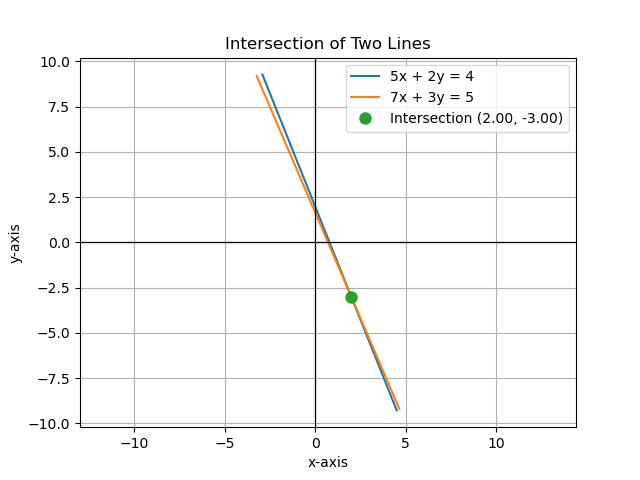
\includegraphics[width=0.7\columnwidth]{figs/Figure_1.png}
    \label{fig:placeholder}
    \caption{1}
\end{figure}
\end{frame}
\end{document}